\chapter{Implementation}
This chapter focuses mainly about the software implementation for semi-automated detection of sanitization, authentication and declassification errors in UML state charts. Used Eclipse xtext to develop source code editor, Eclipse xtend to develop source code generator, YAKINDU SCT editor for modeling C/C++ programs as UML statchart and extended static analysis engine named smtcodan using Java, Graphics2D and JFrame. 

\section{Overview of System Architecture}

A system architecture is the conceptual model that defines the structure, behavior and more views of a system. An architecture description is a formal description and representation of a system, organized in a way that supports reasoning about the structures and behaviors of the system. System architecture is similar to one of the building architecture and it's a global model of this system consisting of a structure, properties (of various elements involved), relationships (between various elements), behaviors and dynamics and multiple views of the system (complementary and consistent).

System Architecture is based on nine fundamental principles:
\begin{itemize}
	\item The objects of the reality are modeled as systems.
	\item A system can be broken down into a set of smaller subsystems, which is less than the whole system.
	\item A system must be considered in interaction with other systems.
	\item A system must be considered through its whole lifecycle.
	\item System can be linked to another through an interface, which will model the properties of the link.
	\item A system can be considered at various abstraction levels, allowing to consider only relevant properties and behaviors.
	\item A system can be viewed according to several layers (usually three: its sense, its functions, and its composition).
	\item A system can be described through interrelated models with given semantics (properties, structure, states, behaviors, data's etc.).
	\item A system can be described through different viewpoints corresponding to various actors concerned by the system.
\end{itemize}

The architecture of our system is given below:
\begin{figure}[!htb]
	\centering
	\vspace{-1em}
	\makebox[\textwidth]{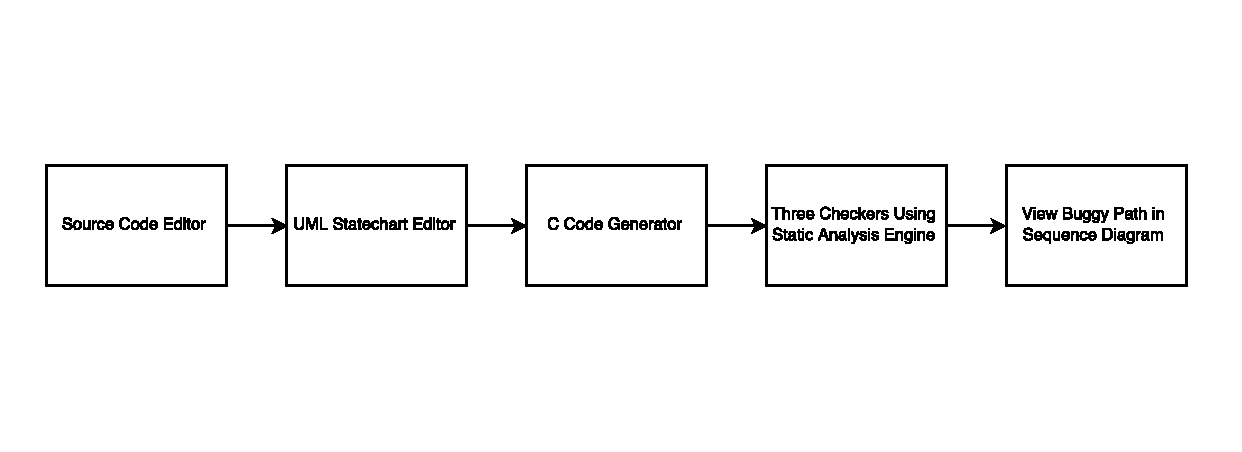
\includegraphics[scale=.50,width=\textwidth]{styles/system_architecture.pdf}}
	\vspace{-5em}
	\caption{System overview}
	\vspace{-1em}
	\label{system_architecture}
\end{figure}

Figure \ref{system_architecture} depicts the complete system overview. At first which is presented as number \circled{1}, the source code editor is developed using Eclipse Xtext. By this editor one can easily annotate the source code of C/C++. It is possible to annotate C/C++ header files. For information flow vulnerabilities detection in C/C++ code, this annotation technique has been chosen which is easy to extend and backward compatible. This editor has been developed as an Eclipse plug-in. If this plug-in exists in eclipse then a user can easily annotate C/C++ source code files and header files by pressing the keys ctrl+space in keyboard. Then for modeling purpose open source tool Yakindu SCT editor \cite{ref_15_yakindu:sct} has been chosen to model the C/C++ code into state charts to detect the bug during design stage of software development life-cycle which is depicted as number \circled{2} in the Figure \ref{system_architecture}. Inside the Yakindu SCT editor the annotation language grammar has also been included using Eclipse Xtext. So, a user can easily annotate the state charts to detect the information flow vulnerabilities. Afterwards the C code generator has been extended inside the Yakindu SCT editor using Eclipse Xtend. This C code generator is represented as number \circled{3} in the Figure \ref{system_architecture}. After modeling, the C code files in Yakindu SCT editor user can easily generate the code using C code generator. Through this generator two files will be generated. One file has .c extension and another file has .h extension. Inside those files annotation has also included. Those annotations are helpful to detect the information flow errors. After generating the code files using static analysis engine named \enquote{smtcodan} three checkers have included to detect authentication, declassification and sanitization function missing vulnerabilities. This three checkers are represented as number \circled{4} phase in the Figure \ref{system_architecture}. Inside the static analysis engine according to the requirements new modules are added. Then to view the buggy path in sequence diagram a sequence diagram generator has been created. Sequence diagram generator to view buggy path is the number \circled{5} and last phase of the system. That is the end of complete system architecture of this system. 


\section{The Grammar of Our Annotation Language}

The goal of the annotation language is to convey library-specific information to the compiler in a simple declarative manner. While it is clear that more sophisticated specifications could support more sophisticated optimizations, our goal is to show that a few simple annotations can enable many useful optimizations. Simplicity is important because we expect our language users to be library experts who do not necessarily have expertise in compilers or formal specifications.

An annotation is meta-data (e.g., a comment, explanation, presentational markup) attached to text, image, or other data. Often, annotations refer to a specific part of the original data. Markup languages like XML and HTML annotate text in a way that is syntactically distinguishable from that text. They can be used to add information about the desired visual presentation, or machine-readable semantic information. If annotations are to be machine-readable, they must have a well-defined syntax. Annotations also need a well-defined semantics. Quite a few specification languages have been defined over the past several decades. 

A special case is the Java programming language, where annotations can be used as a special form of syntactic metadata in the source code. Classes, methods, variables, parameters and packages may be annotated. The annotations can be embedded in class files generated by the compiler and may be retained by the Java virtual machine and thus influence the run-time behavior of an application. It is possible to create meta-annotations out of the existing ones in Java.

The "annotate" function (also known as "blame" or "praise") used in source control systems such as Git, Team Foundation Server and Subversion determines who committed changes to the source code into the repository. This outputs a copy of the source code where each line is annotated with the name of the last contributor to edit that line (and possibly a revision number). This can help establish blame in the event a change caused a malfunction, or identify the author of brilliant code.

For example, Standard Annotation Language or SAL \cite{ref_51_microsoft:sal} is a meta-language that can help static analysis tools, such as analyze switch in Visual Studio 2005 Team System and Visual Studio 2005 Team Edition for Developers, find bugs including security bugs in your C or C++ code at compile time.

Using SAL is relatively easy. User simply add annotations to user's function prototypes that describe more contextual information about the function being annotated. This can include annotations to function arguments and to function return values. The initial focus of SAL is to annotate functions that manipulate read and write buffers. 

\begin{table}
	\centering
	\begin{tabular}{|l|c|p{5cm}|}
		\hline
		\textbf{Category} & \textbf{Parameter Annotation} & \textbf{Description}  \\
		\hline
		
		Input to called function        & \_In\_k  		   & Data is passed to the called function, and 
		is treated as read-only\\
		\hline
		
		Input to called function, and output to caller        & \_Inout\_ & Usable data is passed into the function 
		and potentially is modified. \\ \hline
		Output to caller        & \_Out\_ & The caller only provides space 
		for the called function to write to. 
		The called function writes
		data into that space. \\
		\hline
		
		Output of pointer to caller         & \_Outptr\_  & Like Output to caller. The value that's returned by the called function is a pointer.\\ 	\hline
			
	\end{tabular}
	\vspace{1em}
	\caption{Four basic kinds of parameters for Standard Annotation Language (SAL)}
	\label{table:four basic kinds of parameters}
\end{table}

These four basic annotations in table \ref{table:four basic kinds of parameters}, can be made more explicit in various ways. By default, annotated pointer parameters are assumed to be required, they must be non-NULL for the function to succeed. The most commonly used variation of the basic annotations indicates that a pointer parameter is optional, if it's NULL, the function can still succeed in doing its work. These annotations helps to identify possible uninitialized values and invalid null pointer uses in a formal and accurate manner. Passing NULL to a required parameter might cause a crash, or it might cause a "failed" error code to be returned. Either way, the function cannot succeed in doing its job.

The main benefit of SAL is that user can find more bugs with just a little bit of upfront work. The process of adding SAL annotations to existing code can also find bugs as the developer questions the assumptions previously made about how the function being annotated works. By this as a developer adds annotations to a function, he/she must think about how the function works in more detail than simply assuming it was written correctly. This process finds assumption flaws. Any bugs found in SAL annotated functions tend to be real bugs, not false positives, which has the benefit of speedier bug triage and code fixes.

In this research, annotation language is developed using Eclipse xtext \cite{ref_17_xtext:grammar}. The goal is to overcome the challenge of not being able to detect implicit and explicit information flow bugs in UML state charts and C code. That is why an annotation language has been chosen
which can be used to annotate UML state charts and code by inserting information flow
restrictions during two software development phases (design
and coding). The idea is that the same annotation language
can be used to add information flow constraints to UML state
charts and code in order to detect information flow errors. The grammar of annotation language is represented as in Extended Backus Naur Form (EBNF) in Figure \ref{language grammar}. The following type face conventions have been used: Italic font for non-terminals, bold typewriter font for literal terminals including keywords.
 
 \begin{figure}[ht!]
 	\centering
 	\begin{tabular}{lll}
 		
 		\footnotesize                       
 		\textit{Ann\_Lang}           &\footnotesize $::=$         &\footnotesize HeaderModel*;       \\ \\
 		
 		\footnotesize
 		\textit{H\_Model}            &\footnotesize $::=$         &\footnotesize \textit{S\_L\_Anno};       \hfill ;single line comment rule   \\     
 		&\footnotesize $\ \vert $    &\footnotesize \textit{M\_L\_Anno};       \hfill ;multi line comment rule    \\ 
 		&\footnotesize $\ \vert $    &\footnotesize \textit{Func\_Ann};       \hfill ;function declaration rule  \\ 
 		&\footnotesize $\ \vert $    &\footnotesize \textit{Attr\_Def};        \hfill ;variable declaration rule  \\ \\
 		\footnotesize  	
 		\textit{S\_L\_Anno}          &\footnotesize $::=$         &\footnotesize \textbf{"//@ @function "},    Func\_Type,              [\textbf{H} $\ \vert $  \textbf{L}];     \\
 		&\footnotesize $\ \vert $    &\footnotesize \textbf{"//@ @parameter "},   p\_Name,  Sec\_Type, Var\_Type,    [\textbf{H} $\ \vert $  \textbf{L}];    \\
 		&\footnotesize $\ \vert $    &\footnotesize \textbf{"//@ @variable "},    v\_Name,  Sec\_Type,     [\textbf{H} $\ \vert $  \textbf{L}];    \\
 		&\footnotesize $\ \vert $    &\footnotesize \textbf{"//@ @preStep "},     pr\_s\_Name,             [\textbf{H} $\ \vert $  \textbf{L}];    \\
 		&\footnotesize $\ \vert $    &\footnotesize \textbf{"//@ @postStep "},    po\_s\_Name,             [\textbf{H} $\ \vert $  \textbf{L}];    \\ \\   
 		\footnotesize            
 		\textit{M\_L\_Anno}          &\footnotesize $::=$         &\footnotesize [\textbf{"/*@ "}],  ["* "],  Func\_Ann,  (\textbf{" @*/"}) \\
 		&\footnotesize $\ \vert $    &\footnotesize ("*"), [" "]*, (\textbf{"@*/"});                  \\ \\
 		\footnotesize        
 		\textit{Func\_Ann}           &\footnotesize $::=$         &\footnotesize \textbf{"@function "},    Func\_Type,              [\textbf{H} $\ \vert $  \textbf{L}];     \\
 		&\footnotesize $\ \vert $    &\footnotesize \textbf{"@parameter "},   p\_Name,  Sec\_Type, Var\_Type,    [\textbf{H} $\ \vert $  \textbf{L}];    \\
 		&\footnotesize $\ \vert $    &\footnotesize \textbf{"@preStep "},     pr\_s\_Name,             [\textbf{H} $\ \vert $  \textbf{L}];    \\
 		&\footnotesize $\ \vert $    &\footnotesize \textbf{"@postStep "},    po\_s\_Name,             [\textbf{H} $\ \vert $  \textbf{L}];    \\ \\                                        
 		\footnotesize                       
 		\textit{Func\_Type}          &\footnotesize $::=$        &\footnotesize \textbf{authentication};\\
 		&\footnotesize $\ \vert $ &\footnotesize \textbf{declassification}; \\
 		&\footnotesize $\ \vert $    &\footnotesize \textbf{sanitization};     \\
 		&\footnotesize $\ \vert $    &\footnotesize \textbf{sink};             \\
 		&\footnotesize $\ \vert $    &\footnotesize \textbf{source};           \\
 		&\footnotesize $\ \vert $    &\footnotesize \textbf{trust\_boundary};  \\ \\
 		\footnotesize                       
 		\textit{Sec\_Type}           &\footnotesize $::=$         &\footnotesize \textbf{confidential};\\
 		&\footnotesize $\ \vert $    &\footnotesize \textbf{source};    \\ \\
 	 
 		\footnotesize    	                   
 		\textit{Var\_Type}           &\footnotesize $::=$        &\footnotesize \textbf{authenticated}; \qquad \Comment{Newly added annotations to annotate variable types}\\
 		&\footnotesize $\ \vert $    &\footnotesize \textbf{declassified};
 		\\
 		&\footnotesize $\ \vert $    &\footnotesize \textbf{sanitized};    \\ \\	
 		
 	\end{tabular}
 	\caption{Light-weight annotation language grammar excerpt \cite{ref_108_paul2015infoflow}}
 	\label{language grammar}
 \end{figure}
 
All main rules are included under \texttt{H\_Model}. This  \texttt{H\_Model} rule contains all rules like \texttt{S\_L\_Anno}, \texttt{M\_L\_Anno}, \texttt{Func\_Ann} and \texttt{Attr\_Def}. Annotation language grammar has two grammar rules named \texttt{S\_L\_Anno} and \texttt{M\_L\_Anno} used for defining security annotations. \texttt{S\_L\_Anno} is used for single line annotation rule. Because of this rule one can easily annotate the variables of C/C++ language in a single line. The \texttt{M\_L\_Anno} rule is used for multiline annotation rule. Normally multiline rule annotation is required for function annotation in C/C++ function declaration. The \texttt{Func\_Ann} and \texttt{Attr\_Definition} rules are used to recognize C or C++ function declarations and variable. The \texttt{Var\_Type} rule is used for variable type which is either for authenticated or declassified or sanitized variable. \texttt{Sec\_Type} rule is used for type of security whether a variable is confidential or not. In \texttt{Func\_Type} rule the type of function is declared. A function can be either one of this like authentication, declassification, sanitization, source or sink.

\section{Inference Rules for Secure Information Flows}

The goal is to prevent the information flow from H (high security level, private) variables to 
L (low security level, public) variables through trust boundaries. The inference rules are implemented
inside our static analysis engine which can handle pointers. Considering the following C if statement, if  \[ a(L) \leq b(H)\] then\{\} else\{\}, where variable \emph{a} has attached the label L and variable \emph{b} has attached the label H.
There could be implicit (the variables inside the \emph{then} or \emph{else} branch do not depend on the values of \emph{a}  or \emph{b}) 
and explicit (the variables inside the \emph{then} or \emph{else} branch depend on the values of \emph{a} or \emph{b}) flows between variables
contained in the \emph{then} or \emph{else} as follows: L to L, H to H, L to H and H to L. If a variable labeled H is used afterwards inside
a trust boundary then a information flow leakages should be reported and a bug report should be created. This situation marks as a forbidden flow which we try to detect.

\begin{figure}[ht!]
	\centering
	\begin{tabular}{ll}    
		\circled{A}\ (data types)   &$\tau ::= $ H    $|$  L  $|$ PreStep $|$ PostStep   \\ 
		\circled{B}\ (phrase types) &$\rho ::=  \tau \ | \ \tau \ var \ | \ \tau \ cmd $ \\
	\end{tabular}
	\vspace{1em}
	\caption{Secure typing system specialized on trust boundaries}
	\label{typing:system1}
\end{figure}

Figure \ref{typing:system1} presents the typing system on which our information flow inference rules, depicted in Figure \ref{inference rules}, are based on. In the first row of Figure \ref{typing:system1},\circled{A}, we define the following data types:
H and L used to attach private and public labels to program
variables (High/private and Low/public) and PreStep and
PostStep used to attach function call ordering labels to
previous and post function calls. Figure \ref{typing:system1}, \circled{B} , presents three types of phrases on which our inference rules are based.

\begin{figure}[ht!]
	
	\centering
	\begin{tabular}{ll} 	         
	   \footnotesize 
		 \circled{0} (INT)           &\footnotesize  $ \gamma  \vdash n :$ L    \\ \\
		
		\footnotesize 
		\circled{1} (VAR)            &\footnotesize  $ \gamma  \vdash x$ : H  $\ var$ \ \ \ if $\gamma(x)$ = H $\ var$  \\ \\
		
		\footnotesize  \circled{2} (R-VAL)     &\footnotesize 
		\inferrule{\gamma \vdash e : \ $H$  \ var}
		{\gamma \vdash e : \ $H$  } \\ \\  
		
	    \footnotesize  \circled{3} (F-CALL-P)   &\footnotesize 
		\inferrule{\gamma \vdash e : \tau  \ ($H$) } 
		{\gamma \vdash  e : \tau_{r}  \ ( $L$ )}  \qquad \Comment{Function: authentication, declassification or sanitization}\\ \\ 		 
		
	\end{tabular}
	\caption{Typing rules specialized to L, H for secure explicit and implicit information flow }
	\label{inference rules}
\end{figure}

Figure \ref{inference rules} depicts secure information flow inference rules
which are based on the Denning \cite{ref_14_denning1976lattice} lattice model and Volpano
et al. \cite{ref_38_volpano:sound}. We used only two security levels (L and H) which
correspond to 0 and 1 whereas one could use multiple levels if
required, (e.g., [\dots, --3, --2, --1, 0, 1, 2, 3, \dots]). The expression $ \gamma \vdash e : H $ , \circled{2}, means that expression e has security level H (High). $ \gamma \vdash e : \tau \ H $ , \circled{3} , means that if
a function call (authentication, declassification or sanitization function) was tagged with the parameter label H and then the label of the parameter is replaced with L after execution. The
inference rules presented in Figure \ref{inference rules} describe how the label(s): \circled{0} L is attached to an integer value, \circled{1} H is attached to a variable, \circled{2} H is passed during a return statement, \circled{3} is used to pass the parameter label H and makes the parameter as L between the parameters of a function call.

\section{UML State Chart Editor}

UML is a standard language for specifying, visualizing, constructing, and documenting the artifacts of software systems. UML was created by Object Management Group and UML 1.0 specification draft was proposed to the OMG in January 1997. UML provides elements and components to support the requirement of complex systems. UML follows the object oriented concepts and methodology. So object oriented systems are generally modeled using the pictorial language. UML diagrams are drawn from different perspectives like design, implementation, deployment etc. UML can be defined as a modeling language to capture the architectural, behavioral and structural aspects of a system.

UML state machine diagrams depict the various states that an object may be in and the transitions between those states. In fact, in other modeling languages, it is common for this type of a diagram to be called a state-transition diagram or even simply a state diagram. A state represents a stage in the behavior pattern of an object and like UML activity diagrams it is possible to have initial states and final states. An initial state, also called a creation state, is the one that an object is in when it is first created, whereas a final state is one in which no transitions lead out of. A transition is a progression from one state to another and will be triggered by an event that is either internal or external to the object.

Statechart diagram defines the states of a component and these state changes are dynamic in nature. So its specific purpose is to define state changes triggered by events. Events are internal or external factors influencing the system. Statechart diagrams are used to model states and also events operating on the system. When implementing a system it is very important to clarify different states of an object during its life time and statechart diagrams are used for this purpose. When these states and events are identified they are used to model it and these models are used during implementation of the system. The main uses of UML state chart are:
\begin{itemize}
	\item To model object states of a system.
	\item To model reactive system. Reactive system consists of reactive objects.
	\item To identify events responsible for state changes.
	\item To forward and reverse engineering.
\end{itemize}

\begin{figure}[htbp]
	\centering
	\makebox[\textwidth]{\frame{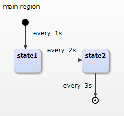
\includegraphics[width=55mm,scale=.55]{styles/simple_statechart.pdf}}}
	\label{fig:simple_stateChart}
	\caption{Simple UML state chart}
\end{figure}

Below are the basic notational elements that can be used to make up a diagram represented in Figure 4.3.
\begin{itemize}
	\item Filled circle, representing to the initial state.	
	\item Hollow circle containing a smaller filled circle, indicating the final state (if any).	
	\item Rounded rectangle, denoting a state.	
	\item Arrow, denoting transition.	
\end{itemize}

Statechart diagram is used to describe the states of different objects in its life cycle. So the emphasis is given on the state changes upon some internal or external events. These states of objects are important to analyze and to implement them accurately. Following are the main purposes of using Statechart diagrams:

\begin{itemize}
	\item To model dynamic aspect of a system.
	
	\item To model life time of a reactive system.
	
	\item To describe different states of an object during its life time.
	
	\item To define a state machine to model states of an object.
\end{itemize}

A set of formal representation of UML state chart is presented in this section. The state identifier and event are represented as S and Event respectively both as set types. For simple specification, the basic set types are used. In the definition of a transition from one state to another the guard is defined as a Boolean type. According to F Alhumaidan state based static and dynamic formal analysis of UML state diagrams \cite{ref_16_alhumaidan2012state} , a state can have three possible values that are active, passive or null represented as Active, Passive and null respectively. The type of state can be simple, concurrent, non-concurrent, initial or final.

\begin{figure}[ht!]
	\centering
	\begin{tabular}{lll}
		\footnotesize                       
		\textit{[S, Event]}          &\footnotesize \\
		
		\footnotesize
		\textit{Boolean}            &\footnotesize $::=$         &\footnotesize \textit{True} $\ \vert $ {False};       \\   
		\footnotesize
		\textit{Status}            &\footnotesize $::=$         &\footnotesize \textit{Active}
		 $\ \vert $ {Passive}$\ \vert $ {Null};       \\ 
		\footnotesize
		\textit{Type}            &\footnotesize $::=$         &\footnotesize \textit{Simple}
		 	$\ \vert $ {Concurent}$\ \vert $ {Nonconcurent} $\ \vert $ {Initial}$\ \vert $ {Final};       \\	 	 
		
	\end{tabular}
	\vspace{1em}
	\caption{UML statechart formal representation}
	\label{statechart_formal_representation}
\end{figure}

In modeling using sets, it is not imposing any restriction upon the number of elements and a high level of
abstraction is supposed. Further, it's not insist upon any
effective procedure for deciding whether an arbitrary
element is a member of the given collection or not. As a
consequence, sets S and Event are sets over which cannot define any operation of set theory. For example,
cardinality to know the number of elements in a set cannot
be defined. Similarly, the subset, union, intersection or
complement operations over the sets are not defined.

The state diagram is a collection of states related by
certain types of relations. In the definition of a state, state identifier, its type, status and set of regions is required. Region is defined as a power set of sequence of states. The state is represented by a schema which consists of four components described above. All these components are encapsulated and put in the Schema State given below.
The invariants over the schema are defined in the second
part of schema.

\begin{figure}[ht!]
	\centering
	\begin{tabular}{lll}
		\footnotesize                       
		\textit{State}       \\
		
		\footnotesize
		\textit{name}   $:$    \textit{S}  \\   
		\footnotesize
		\textit{type}   $:$    \textit{Type}  \\   
		\footnotesize
		\textit{status}   $:$    \textit{Status}      \\
		\footnotesize
		\textit{regions} $:$   \textit{seq Regions} \\
		
		\footnotesize
		\textit{regions} $=$   \textit{1} $\ \  $ {type}$=$   \textit{Simple} \\
		\footnotesize
		 \textit{\# regions} $=$   \textit{1} $\ \  $ {type}$=$   \textit{Nonconcurrent} \\
		 \textit{\# regions} $=$   \textit{1} $\ \  $ {type}$=$   \textit{Concurent} \\
		 
		
	\end{tabular}
	\vspace{1em}
	\caption{More UML statechart formal representation}
	\label{statechart_formal_representation_part2}
\end{figure}

\textbf{Invariants:}
\begin{itemize}
\item  If there is no region in a state inside the state diagram, then it is a simple state.
\item  If there is exactly one region in a state then it is termed as non-concurrent composite state.
\item  If there are two or more regions in a state then it is
concurrent composite state.
\end{itemize}

The collection of states is represented by the schema
States which consists of four variables. The mapping
sub states from State to power set of State describes type
of a state.
 \begin{figure}[ht!]
 	\centering
 	\begin{tabular}{lll}
 		\footnotesize                       
 		\textit{States}          \\
 		\footnotesize                       
 		\textit{start}          
 		$:$  \textit{State}\\
 		
 		\textit{states}          
 		$:$  \textit{State}\\
 		
 		\textit{states}           
 		$:$  \textit{State}\\
 		\footnotesize
 		\textit{substates}            $:$         \textit{State} $\ \  $ {State};       \\   
 		\footnotesize
 		\textit{target}             $:$         \textit{State}    \\
 		 \footnotesize                       
 		 \textit{start}           
 		 $:$  \textit{states}\\
 		  \footnotesize                       
 		  \textit{start}          
 		  $:$ \textit{target}\\
 		   \footnotesize                       
 		   \textit{start}           
 		   $:$  \textit{dom} $\ \  ${substates}\\
 		   
 		   \footnotesize                       
 		   \textit{states}          \\ 		
 		$\ \  $ \textit{s}      $:$     \textit{State} $\ \  $ {s} $\ \  $ \textit{dom} $\ \  ${substates} $\ \  $ {s} $\ \  $ \textit{states}        \\ 
 		$\ \  $ \textit{s}      $:$     \textit{State} $\ \  $ {s} $\ \  $ \textit{states} $\ \  $ {s} $\ \  $ \textit{start} $\ \  $ {s} $\ \  $ \textit{target}$\ \  $ {s.typ}\\ 
 		$\ \  $ \textit{Simple} $\ \  $ {s} $\ \  $ \textit{dom} $\ \  ${substates}\\
 		\footnotesize                       
 		\textit{target}  $\ \  $ \textit{states}        \\ 
 		\footnotesize                       
 		\textit{target}  $\ \  $ \textit{dom} $\ \  ${substates}\\	
 	\end{tabular}
 	\vspace{1em}
 	\caption{UML statechart formal representation for more parts}
 	\label{statechart_formal_representation_invariants}
 	\end{figure}

\textbf{Invariants:}
\begin{itemize}
\item The start state is not in the collection of states.
\item The start state is not the target state.
\item The start state does not belong to domain of substates
mapping that it has no sub-state.
\item For any state, s, if it is in the states and is not the start or target state and not the simple state then it belongs to domain of sub-states.
\item The target state does not belong to states.
\item The target state of the state diagram does not belong to domain of the sub-states.
\end{itemize}

UML state chart editor has been extended based on the open source Yakindu SCT \cite{ref_15_yakindu:sct}framework. The existing language grammar with
annotation language grammar has been extended in order to support new set
of tags. Furthermore, an annotation proposal filter implemented which was used to filter out the annotation language tags of the Yakindu SCT language grammar.

To extend the Yakindu SCT editor here it has been decided to represent the statements e.g. variable declaration, function calling as state and transitions are represent as move from one statement to another. A rectangular box can be attached with transitions where annotation can be written as per requirements. So for the developed system the UML statechart formal representation is as like this: 
\begin{figure}[ht!]
	\centering
	\begin{tabular}{lll}
	\footnotesize                       
	\textit{States}          \\
	\footnotesize                       
	\textit{start}          
	$:$  \textit{State}\\
	
	\textit{states}          
	$:$  \textit{State}\\
	
	\textit{states}           
	$:$  \textit{State}\\
	\footnotesize
	\textit{substates}            $:$         \textit{State} $\ \  $ {State};       \\   
	\footnotesize
	\textit{target}             $:$         \textit{State}    \\
	\footnotesize                       
	\textit{start}           
	$:$  \textit{states}\\
	\footnotesize                       
	\textit{start}          
	$:$ \textit{target}\\
	\footnotesize                       
	\textit{transition}          
	$:$ \textit{annotation*}\\
	\footnotesize                       
	\textit{target} $:$ \textit{states}        \\ 	
	\end{tabular}
	\vspace{1em}
	\caption{UML statechart formal representation for this research}
	\label{statechart_formal_representation_for _this_system}
	\end{figure}
	
\section{Source Code Editor}

A source code editor is a text editor. It is a program which is designed specifically for editing source code of computer programs. It may be built into an integrated development environment (IDE) or web browser. To simplify and speed up input of source code such as syntax highlighting, indentation, autocomplete and bracket matching functionality, source code editors features have designed. Source code editors are the most fundamental programming tool. Some well-known source code editors are Gedit, IntelliJ, NetBeans, Notepad++ and more.

For this research, previous source code editor \cite{ref_108_paul2015infoflow} has been extended which offers annotation language proposals which are context sensitive with respect to the position of the currently edited syntax line. Editor suggestions work only if the whole file is parsed without errors. Editor has been developed using Eclipse Xtext \cite{ref_17_xtext:grammar}.

As per requirements previous annotation language grammar \cite{ref_108_paul2015infoflow} which was written in xtext language has been extended. Extra annotation have included e.g. \enquote{authenticated}, \enquote{declassified}, \enquote{sanitized}, \enquote{sanitization}, \enquote{declassification}, \enquote{authentication}. Mainly FunctionAnnotation, FunctionType  and SingleLineAnnotation rules  are extended. A new rule is added which is enumeration type. The rule name is VariableType. Inside the VariableType new attributes are included e.g. declassified, sanitized and authenticated. New function types are added e.g. declassification, sanitization and authentication function inside FunctionType rule. Inside the FunctionAnnotation and SingleLineAnnotation rules there exist an annotation for parameter name @parameter. Inside @ parameter declaration new attribute is added named VariableType. The code snippet of extended xtext grammar is given in Appendix  \ref{Source_Code_Editor_in_Xtext}. 


From the xtext code snippet previous annotation grammar \cite{ref_108_paul2015infoflow} has FunctionAnnotation(line number 113), SingleLineAnnotation(line number 128) rules. According to the requirements previous rules are extended. Inside the rules of FunctionAnnotation and SingleLineAnnotation, new enumeration types are added. Enumeration type name is VariableType which is declared in line number 172 in \ref{Source_Code_Editor_in_Xtext}. The new enumeration type rule has attributes declassified, sanitized and authenticated. Also the rule of enumeration FunctionType(line number 154 in \ref{Source_Code_Editor_in_Xtext}) extended by adding new type of funtion like authentication, declassification and sanitization.

\section{C Code Generator}
C code generator \cite{ref_108_paul2015infoflow} has been extended based on Eclipse EMF and xTend which is used to generate the state chart execution code containing the previously added security annotations from UML state charts. The code generator outputs two files per UML state chart (one .c and one
.h file). Generated annotations can reside in both header file
and source code file. Previously annotated UML state chart
states are converted to either C function calls or C variables
declarations, both have been previously annotated. The available state chart execution flow functionality has been used which is
responsible for traversing the UML state chart during state
chart simulation. The UML state chart will be traversed by the code generation algorithm and code is generated based on
the mentioned state chart execution flow. The generated code
will contain at least one bad path (contains a true positive) and
a good path (contains no bug) per UML state chart if those
paths were previously modeled inside the UML state chart.

The algorithm \ref{Algorithm:C_Code_Generator} which is given below is representing how the C code generator has developed. The input of the algorithm for code generator is UML statechart. In eclipse xtend \cite{ref_20_xtend} function can be declared as \enquote{def}. Inside the algorithm \ref{Algorithm:C_Code_Generator} the generateTypeH function requires the input of UML statechart. The plug-in named \enquote{MyC} uses eclipse xtend to parse the UML statechart. Inside this function there another two functions named \enquote{typesHAnnotationContent} to generate header file of c(extension .h) and \enquote{typesCAnnotationContent} to generate source code file of c(extension .c). Function typesHAnnotationContent generate the required contents for C header file mostly function signature and annotation of the function which exist in the UML statechart. 

One sample example of a header file of C programming language is given below-

\begin{lstlisting} [caption={C header file codes with annotation},label=lst:cHeaderFileCode]
	/*@ @function authentication
	* @parameter a L @*/
	void authentication(char *a);
	
	/*@ @function source
	* @parameter a L @*/
	void logIn(char *a);
\end{lstlisting}

Inside the algorithm \ref{Algorithm:C_Code_Generator} function typesCAnnotationContent generate the required contents for C source file. This file contains the annotation only for variable declaration. The function annotation is normally located at header file. In this file other code is as normal as C syntax. All functions, statements, variable declaration are similar to C programming language syntax. Inside the function typesHAnnotationContent at first need to get the function annotation as we placed the function signature and function annotation inside the header file. That's why we declared a method named getFileContent who returns a hashmap which contains annotations and statements e.g. variable declaration and function signatures. By iterating the hashmap need to make a check if current statement is not a variable annotation then we placed the annotation and function signatures inside the C header file.

Function typesCAnnotationContent is responsible to generate the C source code. Inside this function to get all function content there is a method called getFunctionContent which returns a hashmap with all function signatures and annotation. By iterating that hashmap the required function signatures are placed inside the C code file. Those functions that have annotations only signatures and blank function bodies are placed inside the C source code file. Because the annotations of the functions mainly placed inside the header file. Now in the modeling stage the system was designed with two regions. One region name is good\_path() and another one is bad\_path(). To get the content of good\_path() and bad\_path(), two methods have created inside the Naming.xtend file named getGoodPathContent() and getBadPathContent(). Those two methods also returned two hashmaps respectively. One hashmap contains the contents of good\_path() region and another hashmap contains the contents of bad\_path() region. Both hashmaps contains the function signatures, statements of C/C++ language and annotations. According to the design in the modeling stage the required contents are placed inside the body of good\_path() and bad\_path(). Normally inside the method of good\_path() and bad\_path() only the variable annotations exist and other statement e.g. function calling, variable declarations etc. The annotations for functions are placed inside the header files of C/C++ language. 

Some of the contents of the header file, C file comes from another xtend file named \enquote{Naming.xtend}. The methods such as getFileContent, getFunctionContent, getGoodPathContent() and getBadPathContent() all are implemented inside the "Naming.xtend" file. The code snippet from C code generator has given in Appendix \ref{C_Code_Generator_Xtend_Code_Snippet_p1} and \ref{C_Code_Generator_Xtend_Code_Snippet_p2}.
\begin{algorithm}
	\label{Algorithm:C_Code_Generator}
	{\textbf{C code generator}}\\
	\noindent\makebox[\linewidth]{\rule{\textwidth}{0.4pt}}
	{\textbf{Input: Statechart}} \\
	{\textbf{Output: .c and .h files}}
	\begin{algorithmic}[1]
	
		\Function{generateTypesH}{$sc$}\Comment{Where sc - statchart}
		
			\State $def {generateFile_1} (testModule.h, typesHAnnotationContent(sc)) $ \Comment{def= function declaration}
			\State $def {generateFile_2} (testModule.c, typesCAnnotationContent(sc)) $  \Comment{C file generator}
		\EndFunction
		
		\Function {typesHAnnotationContent}{$sc$} \Comment{Method for header file generator}		
			\For{$s : getFileContent(sc).entrySet$} \Comment{Iterating hashmap}
				\If {$!s.key.contains('//@ @variable')$} \Comment{Checking not variables}
					\State $s.key$
				\ElsIf {$s.value.contains('(')$} \Comment{Checking functions}
					\State $ void <s.value>;$
				\EndIf		
			\EndFor			
		\EndFunction
		
		\Function {typesCAnnotationContent}{$sc$} \Comment{Method for C file generator}
		
		\For{$s: getFunctionContent(sc).entrySet$}
			\If {$(!s.value.contains('authentication') and (!s.value.contains('declassification'))$  \\  
			$\   \   $   $and(!s.value.contains('sanitization')))$} \Comment{Checking except three types of function}
				\State $void <s.value> {}$
			\EndIf		
		\EndFor
			
		\For{$ region : sc.regions$}
			\If {$ region.name.equalsIgnoreCase('bad\_path()'$} \Comment{Getting the contents of bad path}
			\State $void <region.name>$
				
					\For {$s: getBadPathContent(sc).entrySet$}
					
						\If {$ s.key.contains('//@ @variable')$}  \Comment{Checking variable annotations}
							\State $s.key$
							\State $s.value;$
						\EndIf
					
						\If {$ s.value.contains('(')$} \Comment{Checking function declarations}
							\State $s.value;$
						\EndIf
					
					\EndFor 
			\EndIf
		
			\If {$ region.name.equalsIgnoreCase('good\_path()')$} \Comment{Getting the contents of good path}
			\State $void <region.name>$
				\For {$s: getGoodPathContent(sc).entrySet$} \Comment{Get statements and comments}
					\If {$s.key.contains('//@ @variable')$} \Comment{Check for variable and get the comments} 
						\State $s.key$						
					\EndIf
					\State $s.value;$
				\EndFor 
			\EndIf
				
		\EndFor
				
		\EndFunction
		
		
	\end{algorithmic}
	\noindent\makebox[\linewidth]{\rule{\textwidth}{0.4pt}}
\end{algorithm}

From xtend code snippet in Appendix (\ref{C_Code_Generator_Xtend_Code_Snippet_p1}), xtend can easily access the contents of the state chart which is designed in the modeling stage. For example in case of the function \enquote{getFunctionContent} it parses the function names and put it inside a hash map. It parses those as a function which is a state and contains first bracket e.g. "(". Inside the hashmap it puts the function name and function annotation. In case of the function \enquote{getBadPathContent} which returns the content for the bad path. From the content of state chart there is a region whose name is "bad\_path()". From that region this function parses the comments from each transition and gets the name of each state. Then it puts those contents into a hash map. Through iterating that hashmap according to the algorithm it puts some part of contents in C header file and some part in source code file. The purpose of function \enquote{getGoodPathContent} is to get all the required content from the good path (which is not buggy path). The parameter of this function is the state chart. In the modeling phase it has been declared as a region named "good\_path()". This \enquote{getGoodPathContent} function starts parsing the contents from good path then traverse the whole good path and get all the required contents. After that this function puts the content into a hashmap. This hashmap also contains the function name, function annotation, variable declaration which has annotations. Then according to the algorithm by iterating through the hashmap generates the required files by putting the contents in proper place. 

\section{Three Checkers in Static Analysis Engine}
Static analysis refers to analyzing code without executing it. Generally it is used to find bugs or ensure conformance to coding guidelines. The classic example is a compiler which finds lexical, syntactic and even some semantic mistakes. Static analysis tools should be used when they help maintain code quality. If they are used, they should be integrated into the build process, otherwise they will be ignored. Some characteristics of static analysis tools are:
\begin{itemize}	
	\item Identify anomalies or defects in the code.
	\item Analyze structures and dependencies.
	\item Help in code understanding.
	\item To enforce coding standards.
\end{itemize}

For this research, static analysis engine \enquote{smtcodan}  has been used. Inside the engine, in order to detect the information flow vulnerabilities required classes like AuthenticationFunctionChecker.java, DeclassificationFunctionChacker.java, SanitizationFunctionChecker.Java, Authentication\_gen.java,\\
Declassification\_gen.java,
Sanitization\_gen.java files are included. These files are included in order to detect authentication, declassification and sanitization function missing bug detection in C code. For these three types of function bug detection, here it has been used as library functions in C programming language. In order to detect the information flow vulnerabilities three models have been included such as Authentication\_gen.java,
Declassification\_gen.java,
Sanitization\_gen.java. In the generated .c file there exist these three kinds of methods without signature. As they have no method body that's why they are acting as library function in \enquote{smtcodan} static analysis engine. Inside the engine three function signature will act as keyword like authentication, declassification and sanitization function.

From C code generator, the generated .c and .h file with annotation should act as input for \enquote{smtcodan} static analysis engine. Engine parses the code with annotation. The authentication, declassification and sanitization function all makes the high secured variable or confidential variable as low and according to the policy they pass the information from the sender to the receiver in a secured way. While implementing the checkers, information flow restriction has followed. If any of the C files are not following the secure information flow then bug should be triggered as either authentication , declassification or sanitization function missing function.

\section{View Buggy Path in UML Sequence Diagram}

The Sequence Diagram models the collaboration of objects based on a time sequence. It shows how the objects interact with others in a particular scenario of a use case. A popular use for them is to document the dynamics in an object-oriented system.  For each key collaboration, diagrams are created that show how objects interact in various representative scenarios for that collaboration. An important characteristic of a sequence diagram is that time passes from top to bottom : the interaction starts near the top of the diagram and ends at the bottom. Some of the components of sequence diagram \cite{ref_107_visual-paradigm:visual-paradigm} are described below:

\begin{itemize}
	\item \textbf{Actor:} An Actor models a type of role played by an entity that interacts with the subject (by exchanging signals and data), but which is external to the subject (in the sense that an instance of an actor is not a part of the instance of its corresponding subject). Actors may represent roles played by human users, external hardware, or other subjects. Note that an actor does not necessarily represent a specific physical entity but merely a particular facet (role) of some entity that is relevant to the specification of its associated use cases. Thus, a single physical instance may play the role of several different actors and, conversely, a given actor may be played by multiple different instances.
	
	\item \textbf{Call Message:} A message defines a particular communication between Lifelines of an Interaction. Call message is a kind of message that represents an invocation of operation of target lifeline.
	
	\item \textbf{Create Message:} A message defines a particular communication between Lifelines of an Interaction. Create message is a kind of message that represents the instantiation of (target) lifeline.
	
	\item \textbf{Destroy Message:} A message defines a particular communication between Lifelines of an Interaction. Destroy message is a kind of message that represents the request of destroying the lifecycle of target lifeline.
	
	\item \textbf{Duration Message:} A message defines a particular communication between Lifelines of an Interaction. Duration message shows the distance between two time instants for a message invocation.
	
	\item \textbf{Found Message:} A found message is a message where the receiving event occurrence is known, but there is no (known) sending event occurrence. 
	
	\item \textbf{LifeLine:} A lifeline represents an individual participant in the Interaction.
	
	\item \textbf{Lost Message:} A lost message is a message where the sending event occurrence is known, but there is no receiving event occurrence. We interpret this to be because the message never reached its destination.
	
	\item \textbf{Message:} A message defines a particular communication between Lifelines of an Interaction.
	
	\item \textbf{Return Message:} A message defines a particular communication between Lifelines of an Interaction. Return message is a kind of message that represents the pass of information back to the caller of a corresponded former message.
	
	\item \textbf{Note:} A note (comment) gives the ability to attach various remarks to elements. A comment carries no semantic force, but may contain information that is useful to a modeler.
	
	\item \textbf{Send Message:} A message defines a particular communication between Lifelines of an Interaction. Send message is a kind of message that represents the start of execution.
	
	\item \textbf{Sequence Message:} A message defines a particular communication between Lifelines of an Interaction. Sequence message is a kind of message that represents the need of performing actions in sequence.
	
	\item \textbf{Frame:} A frame represents an interaction, which is a unit of behavior that focuses on the observable exchange of information between connect able elements.
	
	\item \textbf{Concurrent:} A concurrent represents a session of concurrent method invocation along an activation. It is placed on top of an activation.
	
	\item \textbf{Constraint:} A condition or restriction expressed in natural language text or in a machine readable language for the purpose of declaring some of the semantics of an element.
	
	\item \textbf{Continuation:} A Continuation is a syntactic way to define continuations of different branches of an Alternative CombinedFragment. Continuation is intuitively similar to labels representing intermediate points in a flow of control.
	
	\item \textbf{Gate:} A Gate is a connection point for relating a Message outside an InteractionFragment with a Message inside the InteractionFragment.
	
	\item \textbf{Alternative Combined Fragment:} A combined fragment defines an expression of interaction fragments. A combined fragment is defined by an interaction operator and corresponding interaction operands. Through the use of CombinedFragments the user will be able to describe a number of traces in a compact and concise manner.
	
	\item \textbf{Recursive Message:} A message defines a particular communication between Lifelines of an Interaction. Recursive message is a kind of message that represents the invocation of message of the same lifeline. Its target points to an activation on top of the activation where the message was invoked from.
	
	\item \textbf{Self Message:} A message defines a particular communication between Lifelines of an Interaction. Self message is a kind of message that represents the invocation of message of the same lifeline.
	
	\item \textbf{Terminate Message:} A message defines a particular communication between Lifelines of an Interaction. Terminate message is a kind of message that represents the termination of execution.
	
	\item \textbf{Interaction Use:} An InteractionUse refers to an Interaction. The InteractionUse is a shorthand for copying the contents of the referred Interaction where the InteractionUse is. To be accurate the copying must take into account substituting parameters with arguments and connect the formal gates with the actual ones.
	
	\item \textbf{Time Constraint:} A TimeConstraint defines a Constraint that refers to a TimeInterval.
	
	\item \textbf{Uninterpreted Message:} A message defines a particular communication between Lifelines of an Interaction. Uninterpreted message is a kind of message that represents an uninterpreted call.
	
	
\end{itemize}

In this research we used sequence diagram to view the buggy path. In our case, the sending messages are function calls. One function call used to move from one lifeline to another lifeline. We used statements (with line number and file name) before function call into the lifeline which will help the user to trace the buggy path easily.

\begin{figure}[htbp]
	\centering
	\makebox[\textwidth]{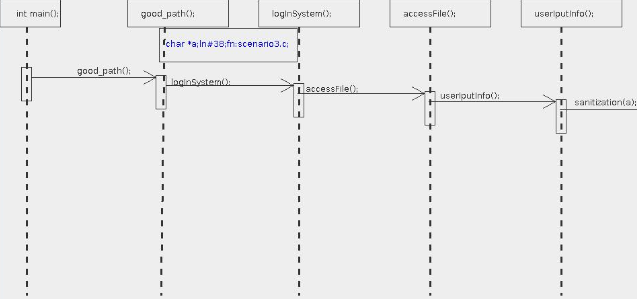
\includegraphics[width=150mm,scale=.50]{styles/newSDDiagram1.pdf}}
	\label{figure:Error_trace_path}
	\caption{Error trace path in UML sequence diagram}
\end{figure}

Through the static analysis engine a buggy path can be found as a list of string. Inside the list there are function calls, separate statements like if statements, switch-case statements, variable declaration, assignment of variables of programming language (e.g. C/C++). Then to view the path using java a sequence diagram is generated. Inside the sequence diagram all function calls are included inside rectangular box attached to the head of lifeline. To switch one lifeline to another a function call required. Like in the Figure 4.8 from function call int main() there is a transition to move from int main() to good\_path(). Above the transition there also exists the function name for which it goes from one function call to another. Here, for example to move from int main() to good\_path() there is a transition and above that transition function call good\_path() is attached. This means through calling the good\_path() function buggy path goes into good\_path() function from int main(); Inside the sequence diagram the statements before the function call are attached to the lifeline as blue color. Those statements are just the statements before a function of the analyzed C/C++ source code file. Inside the box of the blue color texts there exist "ln:" which means the line number of the statement in the analyzed file and "fn:" means the file name of analyzed file. Now it is easier to trace the buggy path by viewing generated sequence diagram. One sample example of the part of a buggy path has given in Figure 4.8.


The process of creating sequence diagram using Java programming language is given below as an algorithm representation. To develop the sequence diagram, a separate class is included inside the smtcodan project. The class name is SequenceDiagramGenerator. Inside this class the drawSequenceDiagram function creates the diagram. The function input parameter is a list of IASTNode which is delivered from the smtcodan project packages. To draw the diagram BufferedImage, Graphics2D, JPanel, JFrame  classes were used. At first it is required to declare object for each of these (BufferedImage, Graphics2D, JPanel, JFrame) classes. Then iterating through the list of IASTNodes set all the statements except function call with line number and file name. There is a class which is responsible to draw the visual things of the sequence diagram named MyCanvasDraw. Afterwards it is required to create an object of this class. This class has a list. The list of this class has to be set with the list of all statements, line number  and file name. Then it will draw the diagram according to the list. To view this diagram need to set the JFrame object and make it visible. Inside the JFrame JScrollpane object also added to make the frame scrollable. For saving the diagram as an image save as option is also included. Through the menu bar, user can easily save the sequence diagram as an image. By default it will save the image as in .jpg format. But one can easily save this image in other format like .png,.bmp,.jpeg etc. Exit option is also included inside the JFrame through which user can exit the current window.  


\begin{algorithm}
	{\textbf{Sequence diagram generator}}\\	
	\noindent\makebox[\linewidth]{\rule{\textwidth}{0.4pt}}
	{\textbf{Input: List of statements and function call}} \\
	{\textbf{Output: Sequence diagram in a frame}}
	\begin{algorithmic}[1]
		
		\Function{drawSequenceDiagram}{$ArrayList<IASTNode> statementsList$}
		    \State $ Frame (object)  $  \Comment{Frame object initialization}
			\State $ BufferedImage (object)  $ \Comment{BufferedImage object initialization}
			\State $ Graphics2D(object) $ \Comment{Graphics2D object initialization}
			\State $ Panel (object)$ \Comment{Panel object initialization}
			\State $ MyCanvasDraw(object )  $ \Comment{MyCanvasDraw object initialization}
			\For{$i:statementsList.size()$} 
				\If {$!statementsList.get(i).getRawSignature().toString().contains("(")$} 
					
					\State $int j=i;$
					\If{$j<=statementsList.size()-2$}
						\State $do$
						\State $add(ln)$ \Comment{ln=line number}
						\State $add(fn)$ \Comment{fn=file name}
						\State $while(!statementsList.get(j).getRawSignature().toString().contains("("))$
						\State $mcd.buggyPathList.add(allStatements);$ \Comment{Where allStatements - statements of C}
					\EndIf				
				\EndIf		
				
			\EndFor
				\State $set <- ScrollPane(property)$ \Comment{Setting ScrollPane property}
				\State $mcd.paint(graphics2D)$ \Comment{Where mcd = MyCanvasDraw object}
				\State $topPanel.add(mcd)$ \Comment{Where topPanel = Panel object}	
				\State $menuBar <- MenuBar$ \Comment{Adding menu bar}
				\State $menuFile <- Menu $
				\State $menuFileExit <- MenuItem$ \Comment{Adding exit menu}
				\State $menuSaveAs <- MenuItem $ \Comment{Adding save as menu}
				\State $menuSaveAs.addActionListener <- fileSave and exit$
				\State $set<-frame (properties=visibility,menubar)$
		
		\EndFunction		
		
	\end{algorithmic}
	\noindent\makebox[\linewidth]{\rule{\textwidth}{0.4pt}}
\end{algorithm}
